\cleardoublepage

\section{服务器端程序实现}
上章主要介绍了文章的研究背景以及国内外对形变传感器、曲线重建算法、三维渲染技术和网络传输技术的研究现状,
并提出了一种改良的曲线重建算法和大致的实现步骤。这些理论和方案的具体实践将会在本章和下一章中介绍。

本章主要介绍服务器端程序的实现。整个服务器端程序都采用Rust编程语言\cite{rust}构建,
Rust是一门C或C++编程语言的替代语言,它速度惊人且内存利用率极高。
由于没有运行时和垃圾回收,它能够胜任对性能要求特别高的服务,可以在嵌入式设备上运行,还能轻松和其他语言集成。
它丰富的类型系统和所有权模型保证了内存安全和线程安全,让您在编译期就能够消除各种各样的错误。
另外,它拥有出色的文档、友好的编译器和清晰的错误提示信息,还集成了一流的工具——包管理器和构建工具,
智能地自动补全和类型检验的多编辑器支持,以及自动格式化代码等等。 

\subsection{数据上推流注册模块}
这个模块需要接收客户端上推的原始数据。所使用的协议为WebSocket on HTTPS。
本文选用的Web Server是hyper\cite{hyper},并基于它实现了一个简单的Web框架roa\cite{roa}。

hyper是一个专注正确性和高性能的http库,但过于底层,使用不便。
roa是一个类koajs\cite{koajs}的web框架,灵活而易于拓展。
数据上推流注册模块基于roa框架的HTTPS和WebSocket支持,给每个注册的数据源分配唯一的id。

数据源注册请求就是一个WebSocket请求:

\begin{lstlisting}[label={lst:register-source},caption={发起数据源注册请求}]
websocket wss://host:port/upstream/
\end{lstlisting}

连接建立之后服务器端给客户端发一个确认包,以告知注册的频道$id$。

\begin{lstlisting}[language=json,firstnumber=1,label={lst:register-resp},caption={数据源注册成功}]
{
    "id": 1
}
\end{lstlisting}

我们采用JSON\cite{rfc7159}作为主要的数据传输序列化格式,这段数据告诉客户端注册频道$id$为$1$,数据上推准备已完成。

其逻辑伪代码如下:

\begin{lstlisting}[caption={注册数据源}]
for connection in incomming() {
    id := sources.push(connection)
    connection.send({"id": id})
}
\end{lstlisting}

其中$incomming$函数接受新的请求连接,$sources$数据源频道列表。
原始数据即传感器直接或间接测得的曲率数据,其内容如代码块 ~\ref{lst:raw-data}中所示。

\subsection{曲线重建模块}
图形学上常用的连续化算法(曲线)有贝塞尔(Bezier)曲线、B样条曲线、Catmull Rom样条曲线等;
而统计学上常用线性插值、多项式插值等。图形学连续化的常见目的是得到光滑曲线,而统计学则追求最小偏差。
由于“曲率光滑程度对曲线重建结果的影响”尚无理论研究,也超出了本文的研究范围,故本文采用其中最简便的线性插值法。

线性插值的实现比较简单,先算出两个方向曲率$k_a$,$k_b$变化的斜率$k_{k_a}$,$k_{k_b}$,
再根据斜率和插值步长$d_s$进行插值。其伪代码如下:

\begin{lstlisting}[caption={线性插值法}]
raw := raws.first()
for next_raw in raws {
    s := next_raw.s - raw.s
    kka := (next_raw.ka - raw.ka) / s
    kkb := (next_raw.kb - raw.kb) / s
    for i in range(0, s / ds) {
        curvatures.push({
            "ka": raw.ka + kka * i, 
            "kb": raw.kb + kkb * i,
        })
    }
    raw = next_raw
}
\end{lstlisting}

其中$raws$为一组原始数据,其每个成员数据都包含一个测量点的弧长曲率数据;
$ds$为采用的插值步长;
$curvatures$为插值后的曲率数据。
得到连续化后的曲率数据 $curvatures$ 如代码块 ~\ref{lst:curvature-vec}中所示。

曲线重建算法需要的运算(如加减乘除、三角函数、平方开方和矩阵运算)Rust语言库均有提供。核心逻辑伪代码如下:

\begin{lstlisting}[caption={曲线重建}]
for ka, kb in curvatures {
    k := sqrt(ka ^ 2 + kb ^ 2)
    theta := k * ds
    cos_alpha := ka / k
    sin_alpha := kb / k
    cos_theta := cos(theta)
    sin_theta := sin(theta)
    da := cos_alpha * (1 - cos_theta) / k
    db := sin_alpha * (1 - cos_theta) / k
    dc := sin_theta / k
    ti = 1 / ri * [da, db, dc]
    ai += ti
    [x, y, z] := ai.column(0)
    points.push(Point {x, y, z})
    // get next rotation matrix
    ri = Matrix3::new(
        cos_alpha, -sin_alpha, 0.,
        sin_alpha, cos_alpha, 0.,
        0., 0., 1.,
    ) * Matrix3::new(
        cos_theta, 0., sin_theta,
        0., 1., 0.,
        -sin_theta, 0., cos_theta,
    ) * Matrix3::new(
        cos_alpha, sin_alpha, 0.,
        -sin_alpha, cos_alpha, 0.,
        0., 0., 1.,
    ) * ri
}
\end{lstlisting}

其中$ri$为旋转矩阵,初始值等于单位矩阵;ti为每个微元内的平移矩阵;ai为总平移矩阵。
重建出的坐标点数据如代码块~\ref{lst:positions}所示。

\subsection{数据下推流订阅模块}

重建数据订阅请求同样是一个WebSocket请求:

\begin{lstlisting}[label={lst:subscribe},caption={重建数据订阅}]
websocket wss://host:port/downstream/:id
\end{lstlisting}

其中的$:id$为频道$id$,在上推数据源注册时获得。
重建数据下推流中的一份数据样例如代码块 ~\ref{lst:positions}所示。
其逻辑伪代码如下:

\begin{lstlisting}[caption={订阅数据源}]
for id, connection in incomming() {
    source := sources.get(id)
    connection.subscribe(source)
}
\end{lstlisting}

\subsection{重建效果与误差分析}

本节主要内容是重建算法的效果展示与误差分析。
为了方便画图和分析,所用曲线为二维标准余弦曲线。

\subsubsection{结果与误差}

图 ~\ref{fig:cos} 为标准余弦曲线与插值步长为$0.01$时的重建结果对比图。
图 ~\ref{fig:cos-error} 展示了根据横坐标$x$变化的重建误差,误差定义为两曲线$y$轴坐标之差的绝对值。

由图可知标准余弦曲线一个周期内的重建误差都在$0.05$以内。


\begin{figure}[H]
\centering
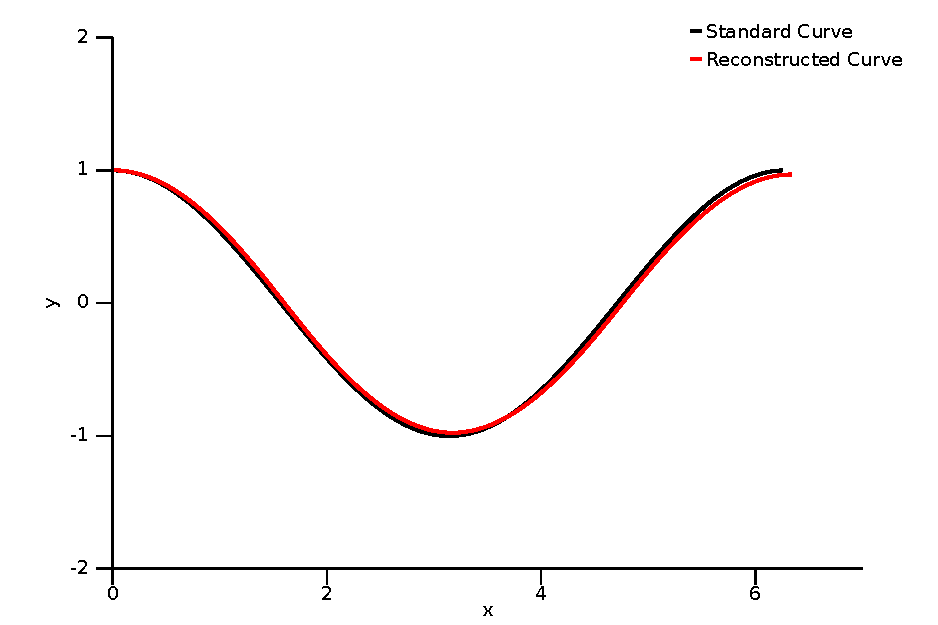
\includegraphics{cos.pdf}
\caption{余弦曲线重建结果}
\label{fig:cos}
\end{figure}

\begin{figure}[H]
\centering
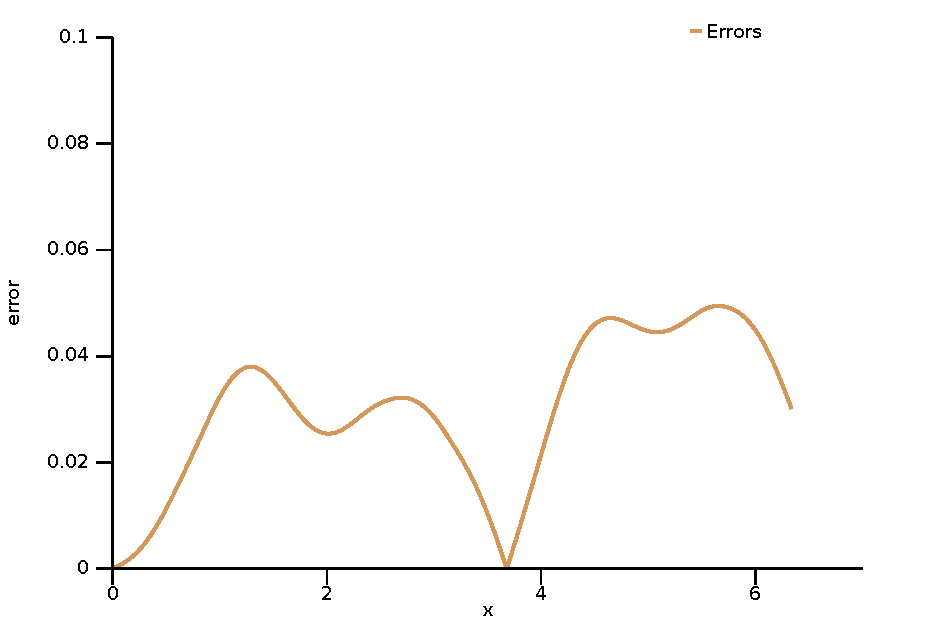
\includegraphics{cos-error.pdf}
\caption{余弦曲线重建误差}
\label{fig:cos-error}
\end{figure}

\subsubsection{不同步长下的误差}

图 ~\ref{fig:cos-diff-step} 为标准余弦曲线与不同插值步长的重建结果对比图。
图 ~\ref{fig:cos-diff-step-error} 展示了横坐标$x$变化下不同插值步长的重建误差。

可知步长越小重建误差越小,但步长从$0.01$减少到$0.001$带来的准确性提升并不是很明显,却增加了十倍的计算负担,
故可认为$0.01$为最适插值步长。

\begin{figure}[H]
\centering
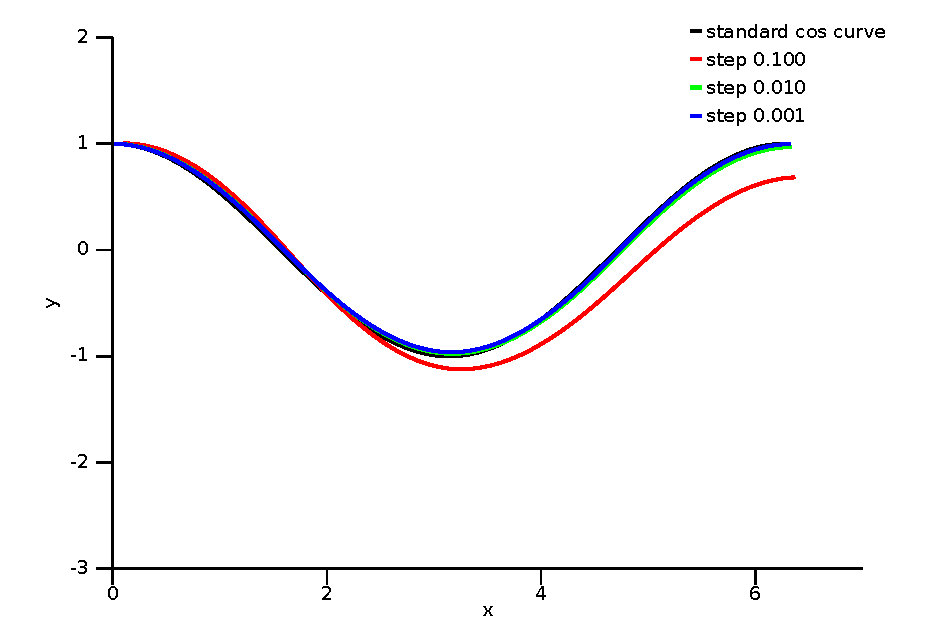
\includegraphics{cos-diff-step.pdf}
\caption{不同步长下的重建结果}
\label{fig:cos-diff-step}
\end{figure}

\begin{figure}[H]
\centering
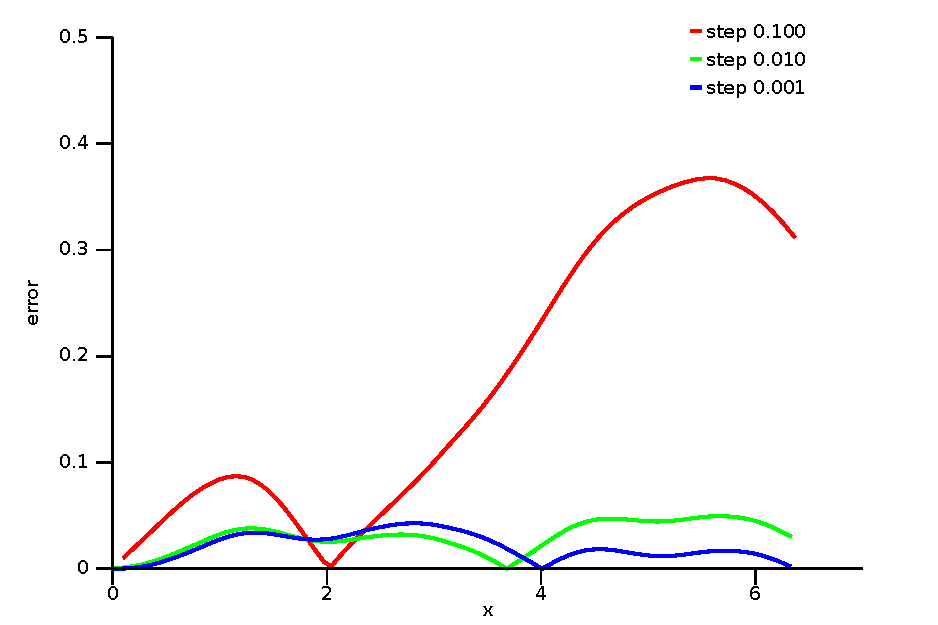
\includegraphics{cos-diff-step-error.pdf}
\caption{不同步长下的重建误差}
\label{fig:cos-diff-step-error}
\end{figure}

\subsubsection{误差传递}

图 ~\ref{fig:cos-single-error-view} 为$x = \frac{\pi}{4}$处加入不同曲率数据误差的重建结果,曲率误差的定义为原始曲率的倍数。
图 ~\ref{fig:cos-single-error} 展示了横坐标$x$变化下加入单点曲率误差的的重建误差传递。

可知单点曲率误差越大重建误差也越大,
且每增加$0.1$倍的曲率误差对重建结果的影响都是巨大的,故原始曲率数据的准确性十分重要。

\begin{figure}[H]
\centering
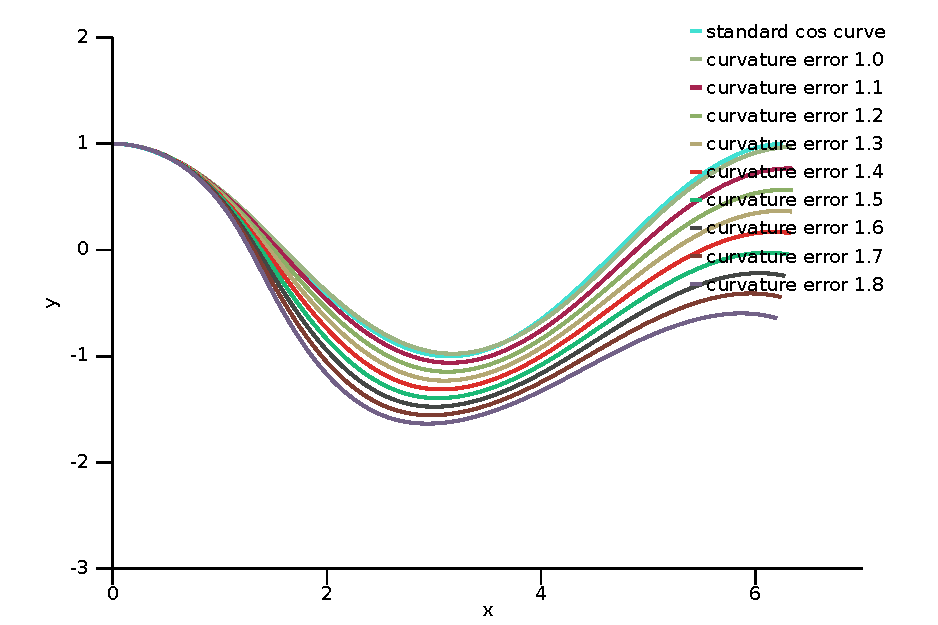
\includegraphics{cos-single-error-view.pdf}
\caption{加入单点误差的重建结果}
\label{fig:cos-single-error-view}
\end{figure}

\begin{figure}[H]
\centering
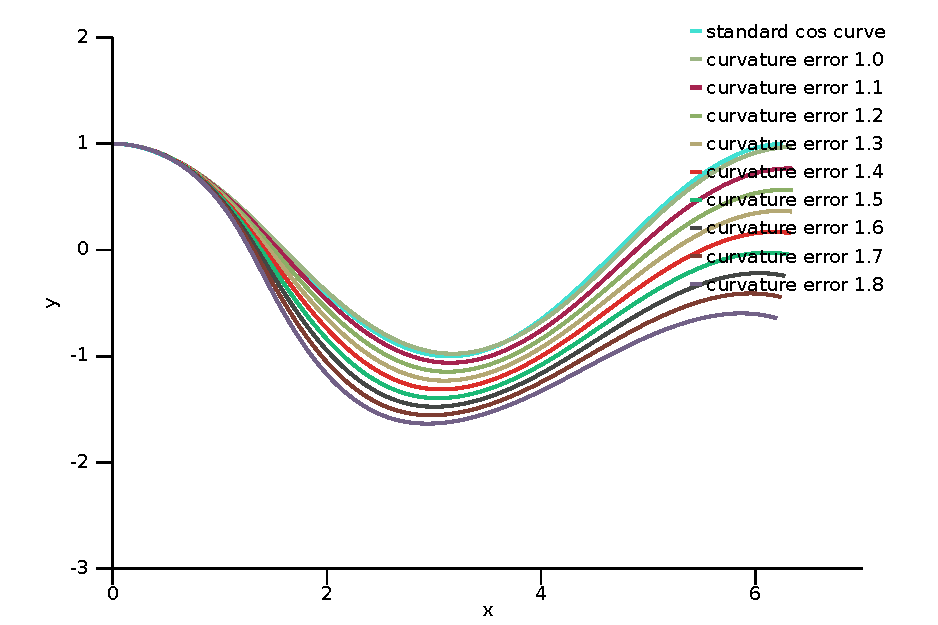
\includegraphics{cos-single-error.pdf}
\caption{单点误差的传递}
\label{fig:cos-single-error}
\end{figure}

图 ~\ref{fig:cos-multiple-error-view} 为曲线上多点分别加入$1.2$曲率数据误差的重建结果。
图 ~\ref{fig:cos-multiple-error} 展示了横坐标$x$变化下分别加入多点曲率误差的的重建误差传递。

可知$s=4.672$处引入曲率误差对重建结果的影响最小,而$s=0.000$处引入对整体曲线影响最大,
但$s=3.820$处引入对后半段曲线的重建结果影响最大,总体来说没什么规律可循。

\begin{figure}[H]
\centering
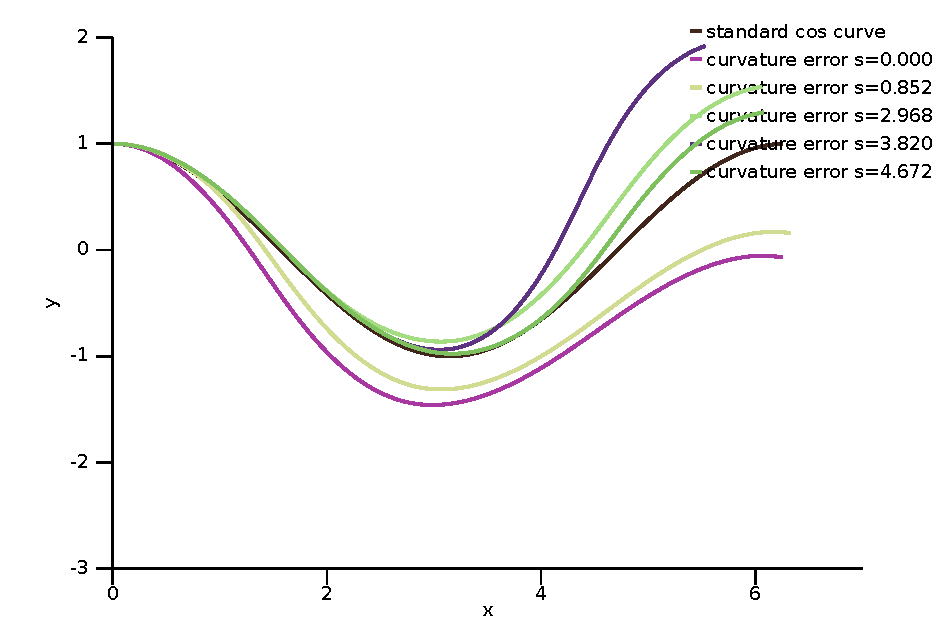
\includegraphics{cos-multiple-error-view.pdf}
\caption{加入多点误差的重建结果}
\label{fig:cos-multiple-error-view}
\end{figure}

\begin{figure}[H]
\centering
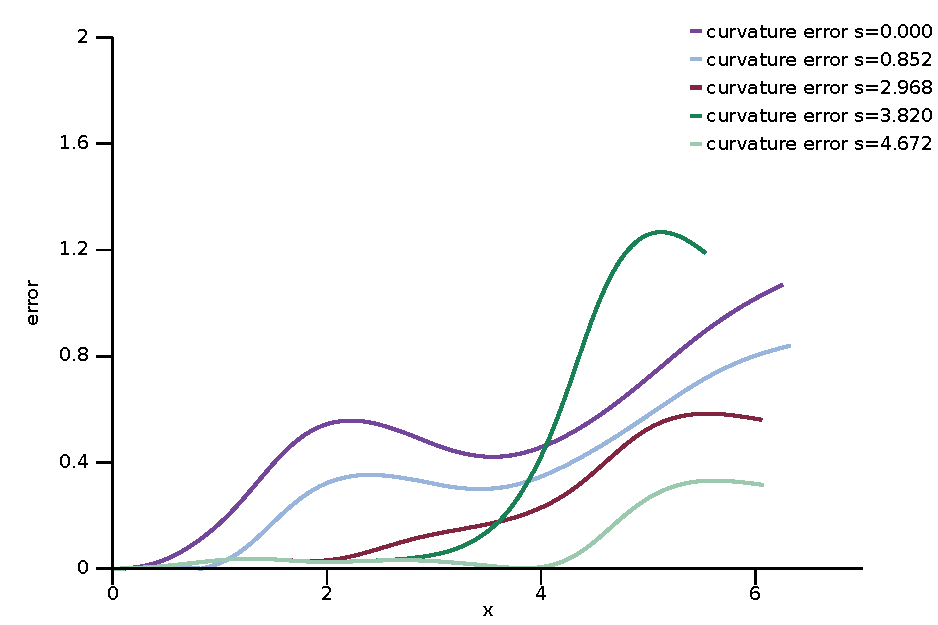
\includegraphics{cos-multiple-error.pdf}
\caption{多点误差的传递}
\label{fig:cos-multiple-error}
\end{figure}

\cleardoublepage

\section{客户端程序实现}
上章主要介绍了服务器端程序的实现,包括数据上推流注册、曲线重建和数据下推流订阅三个模块。
其中数据上推流注册和数据下推流订阅两个功能均需要相应客户端的支持。
本章主要介绍两个客户端程序的实现,它们分别是原始数据推流客户端和渲染客户端。

\subsection{原始数据推流客户端}
原始数据推流客户端需要直接获得原始曲率数据,对性能的要求不高,但需要支持TCP网络栈。
权衡价格、能耗、易用性等因素,本文使用运行Linux系统的树莓派机器。
Linux平台同样支持Rust编程语言,可以使用hyper客户端的WebSocket扩展库。

原始数据推流客户端程序核心逻辑如下:

\begin{enumerate}
\item \textbf{注册数据源:}如代码块~\ref{lst:register-source}和~\ref{lst:register-resp}所示;
\item \textbf{上推数据:} \\
伪代码如下:

\begin{lstlisting}[caption={上推数据}]
for raw_data in sense() {
    connection.send(raw_data)
}
\end{lstlisting}

其中$sense$函数会持续地返回原始数据,之后再通过WebSocket连接将数据发往服务器端。

\end{enumerate}

\subsection{渲染客户端}

渲染客户端的主要功能是根据服务器下推的点列实时渲染管壁或轴线。
三维渲染采用WebGL渲染引擎和Threejs库,
WebGL是浏览器上的OpenGL实现,用于在任何兼容的Web浏览器中呈现交互式3D和2D图形\cite{webgl}。
WebGL通过引入一个与OpenGL ES 2.0紧密相符合的API,可以在HTML5<canvas>元素中使用。

目前支持WebGL的浏览器有:Firefox 4+、Google Chrome 9+、Opera 12+、Safari 5.1+和Internet Explorer 11+;
但是WebGL一些特性也需要用户的硬件设备支持。

WebGL几乎是完全地“跨平台”,使用任何支持WebGL的浏览器打开网页即可完成客户端渲染,而无需下载另外的软件或浏览器插件。

Three.js是一个基于WebGL的3D图形库\cite{threejs},它封装了很多实用的图形组件。

\subsubsection{数据订阅模块}
渲染流程的第一步是向服务器订阅重建的坐标数据,并根据坐标数据拟合一条Catmull Rom曲线。
数据订阅请求使用浏览器提供的WebSocket接口\cite{mdn-websocket},
曲线拟合使用Threejs提供的$CatmullRomCurve3$。

数据订阅流程如下:

\begin{enumerate}
\item \textbf{订阅数据源:}如代码块~\ref{lst:subscribe}所示;
\item \textbf{接收数据:} \\
重建坐标数据的格式见代码块 ~\ref{lst:positions},逻辑伪代码如下:

\begin{lstlisting}[caption={订阅数据}]
for points in receive() {
    curve := new CatmullRomCurve3(points)
}
\end{lstlisting}

其中$receive$函数会持续地接收坐标数据$points$,之后再基于坐标数据拟合曲线。

\end{enumerate}

\subsubsection{轴线渲染}

获得曲线之后,先考虑渲染一条轴线。
三维渲染的一条线是不需要考虑直径等几何属性的,只需要指定基曲线和基础线材料即可完成渲染。
基础线材料采用Threejs提供的$LineBasicMaterial$,并另外使用其提供的$BufferGeometry$作为动态曲线的缓冲区。
伪代码如下:

\begin{lstlisting}[caption={渲染轴线}]
material := new LineBasicMaterial()
bufGeometry := new THREE.BufferGeometry()
object := new Line(bufGeometry, material)
for points in receive() {
    curve := new CatmullRomCurve3(points)
    bufGeometry.setCurve(curve)
}
\end{lstlisting}

\subsubsection{管壁渲染}

管壁是一个三维物体,它有固定的直径等几何属性和反光度等材料属性,构建过程比轴线更复杂。

本文使用Threejs提供的$MeshPhongMaterial$材质,它是一种光亮的材质,可以模拟具有镜面高光的光泽表面。
渲染一个使用网格材质,双边渲染,分段数$64$,直径$0.1$,反光度$100$的管壁伪代码如下:

\begin{lstlisting}[caption={渲染管壁}]
material := new MeshPhongMaterial({
    shininess: 100,
    side: THREE.DoubleSide,
})
geometry = new TubeGeometry(curve, 64, 0.1)
object := new Mesh(geometry, material)
\end{lstlisting}

\subsubsection{控制器}
控制器是一种响应外部输入(如鼠标键盘)以控制摄像头或其它物体位置、大小、形状的程序模块。
本文主要使用的控制器为轨道控制器,摄像头可以响应鼠标动作绕某一点三轴旋转、缩放,
或是响应键盘上下左右键平移。

轨道控制器使用Threejs提供的$OrbitControls$,其围绕原点旋转伪代码如下:

\begin{lstlisting}[caption={轨道控制器}]
orbitControls := new OrbitControls(camera)
orbitControls.target = [0, 0, 0]
\end{lstlisting}

\subsubsection{环境光}

没有施加环境光照的情况下摄像头是拍不到任何图像的。常用的环境光主要有三类:全局光、平行光和点光源。
全局光均匀地照射在场景的每一个物体上,不会产生阴影或者反光,非常易于计算但过于朴素;
平行光会产生阴影和反光效果,并且相对易于计算;点光源计算难度较大,但视觉效果较好。

本文使用一个RGB颜色为$\#111111$的全局光和一个颜色为$\#505050$的点光源组成复合光源,
点光源位于空间中坐标$[0, 1000, 0]$处。
全局光和点光源分别使用Threejs提供的$AmbientLight$和$DirectionalLight$,
伪代码如下:

\begin{lstlisting}[caption={环境光}]
scene.add(new AmbientLight(0x111111))
spotLight := new DirectionalLight(0x505050)
spotLight.position.set(0, 1000, 0)
scene.add(spotLight)
\end{lstlisting}

\cleardoublepage

\section{软件运行展示}
第一章中介绍了一种改良的重建算法和曲线重建可视化的实现步骤,
第二章和第三章分别介绍了服务器端和客户端程序的实现细节。
本章将介绍客户端与服务器端对接后,软件整体的使用说明和渲染效果。
展示所用曲线为$[0, 2\pi]$区间内的动态三维余弦曲线,
实时动态展示网址:\href{https://curve.hexilee.me:8000/}{https://curve.hexilee.me:8000/}。

\subsection{使用说明}

图 ~\ref{fig:tube-default} 是软件的默认渲染结果。
\begin{figure}[H]
\centering
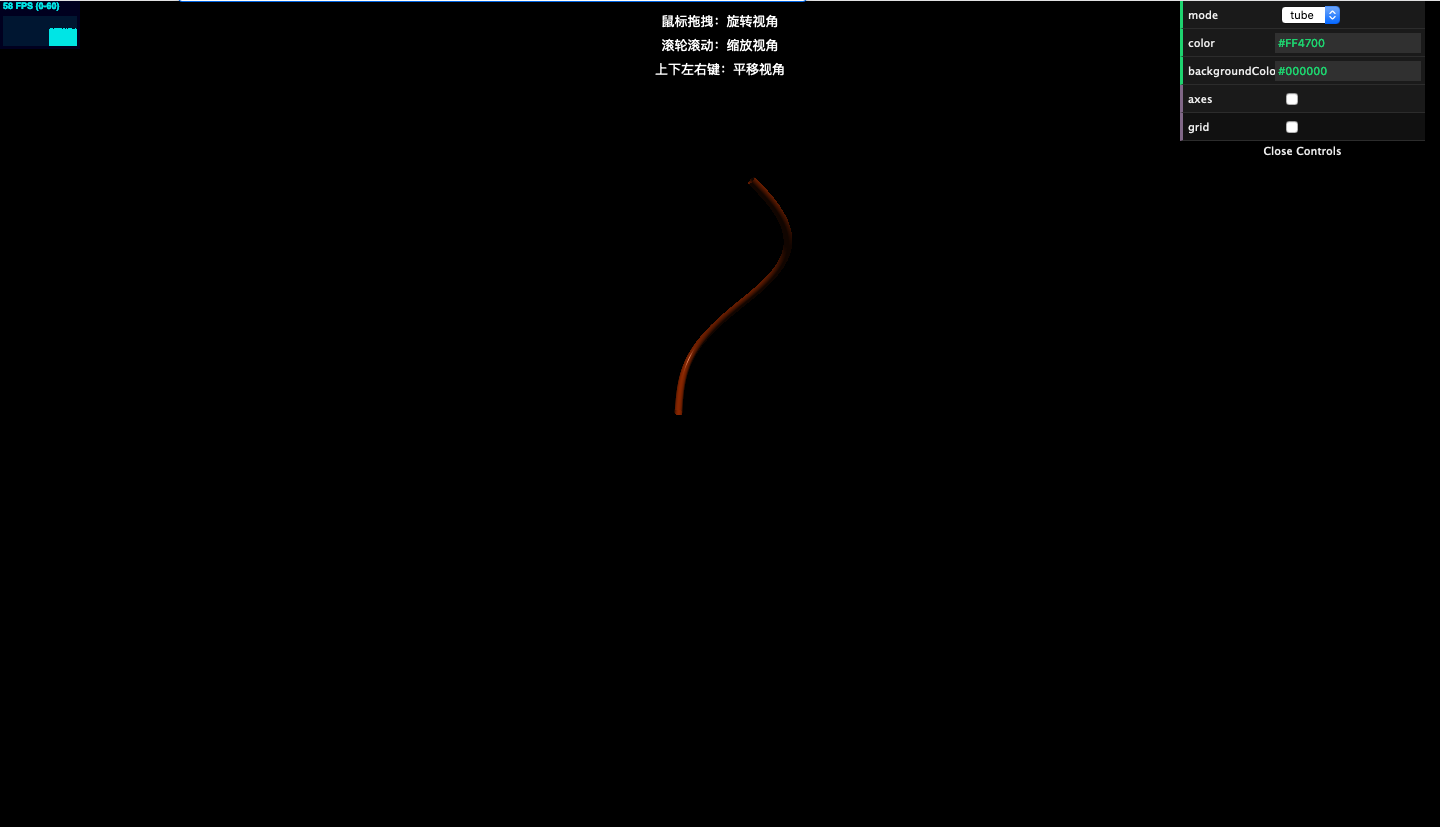
\includegraphics[scale=0.3]{tube-default.png}
\caption{管壁渲染}
\label{fig:tube-default}
\end{figure}

界面左上角是帧率监控,如图 ~\ref{fig:fps} 表示帧率区间$18-60$,当前帧率$60$。

\begin{figure}[H]
\centering
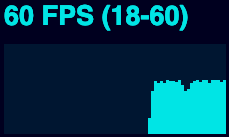
\includegraphics[scale=0.3]{fps.png}
\caption{帧率监控}
\label{fig:fps}
\end{figure}

界面顶端为交互说明:

\begin{itemize}
\item 鼠标拖拽:旋转视角
\item 滚轮滚动:旋转视角
\item 上下左右键:平移视角
\end{itemize}

界面右上角为控制面板,用于控制渲染选项。
如图 ~\ref{fig:control-pad} 为默认选项,各选项的可选值和含义分别为:

\begin{enumerate}
\item \textbf{mode: }渲染模式,可选择管壁渲染或者轴线渲染;
\item \textbf{color: }轴线或管壁的颜色,手动填入十六进制RGB值;
\item \textbf{backgroundColor: }背景颜色,手动填入十六进制RGB值;
\item \textbf{axes: }勾选显示坐标轴;
\item \textbf{grid: }勾选显示辅助栅格;
\end{enumerate}

\begin{figure}[H]
\centering
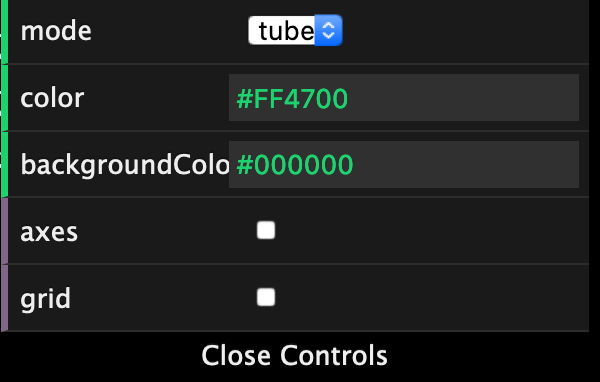
\includegraphics[scale=0.3]{control-pad.png}
\caption{控制面板}
\label{fig:control-pad}
\end{figure}

\subsection{渲染效果}
上一节中我们展示了默认的渲染效果并介绍了软件界面和使用说明,
本节将会展示在各种选项下的渲染效果。

\begin{enumerate}

\item \textbf{轴线渲染} \\
渲染模式$mode$切换到选项$line$:

\begin{figure}[H]
\centering
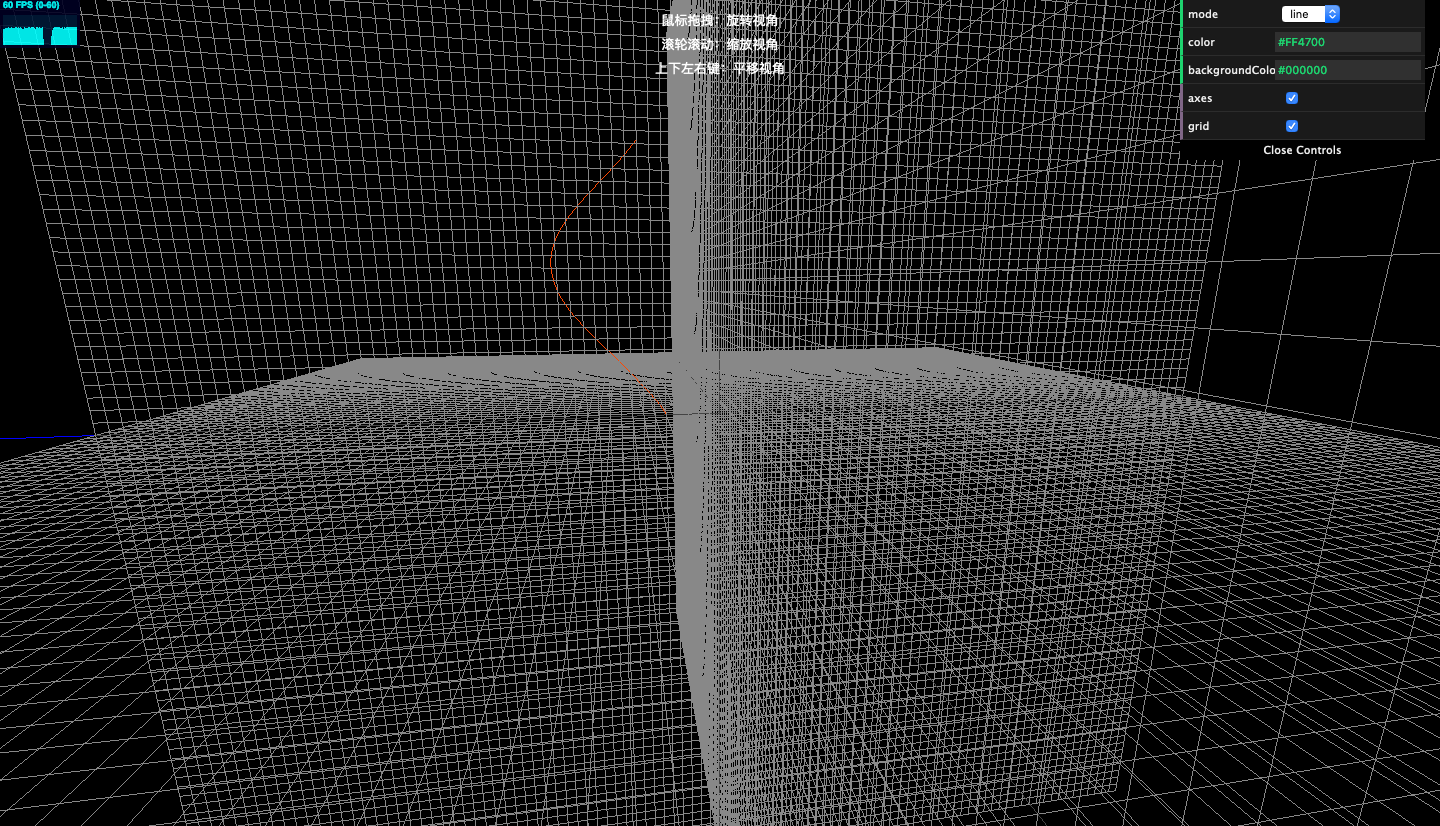
\includegraphics[scale=0.3]{line.png}
\caption{轴线渲染}
\label{fig:line}
\end{figure}

\item \textbf{改变管壁颜色} \\
改变管壁颜色为$\#00FFFF$:

\begin{figure}[H]
\centering
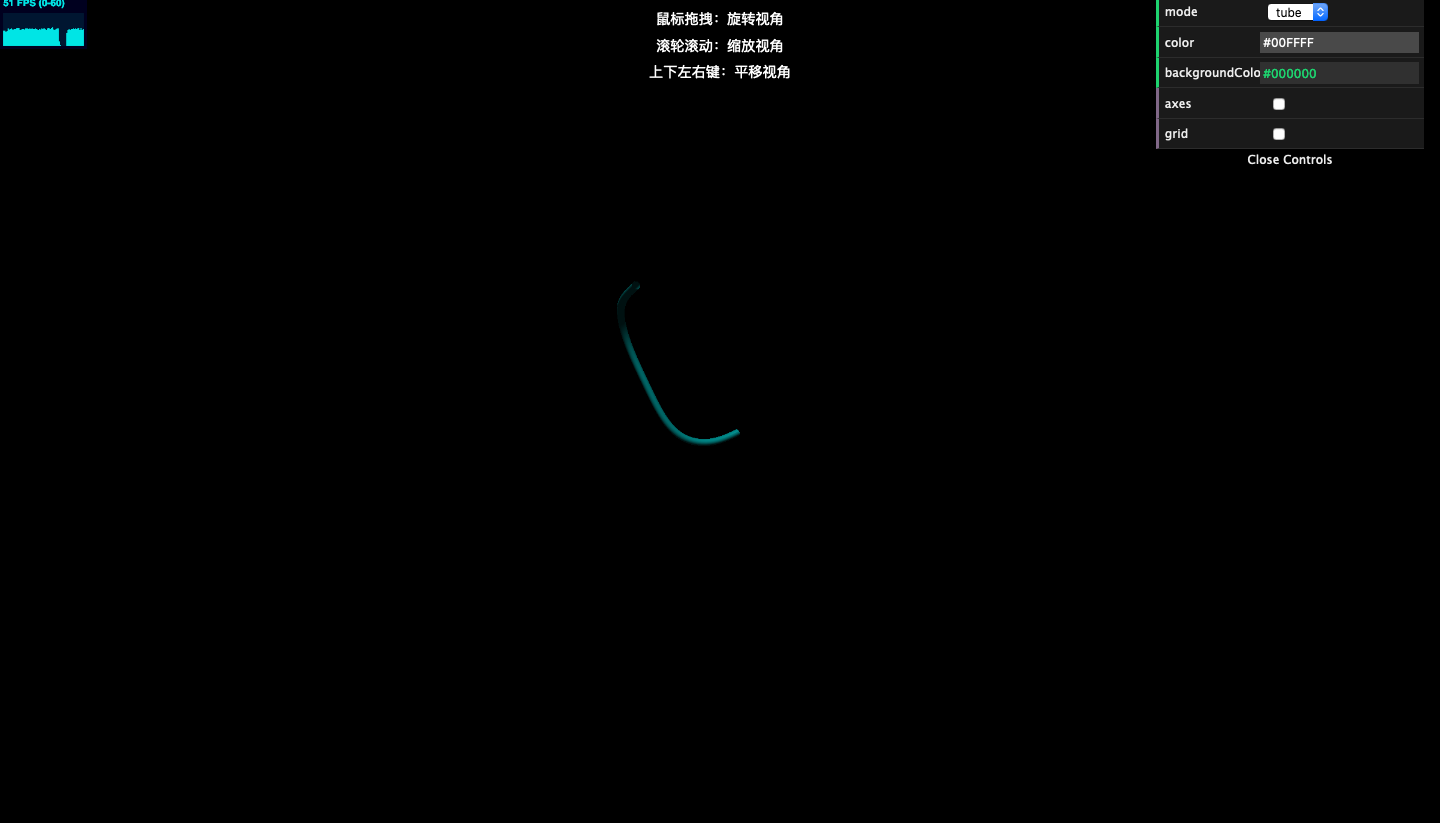
\includegraphics[scale=0.3]{change-color.png}
\caption{改变管壁颜色}
\label{fig:change-color}
\end{figure}

\item \textbf{改变背景颜色} \\
改变背景颜色为$\#222222$:

\begin{figure}[H]
\centering
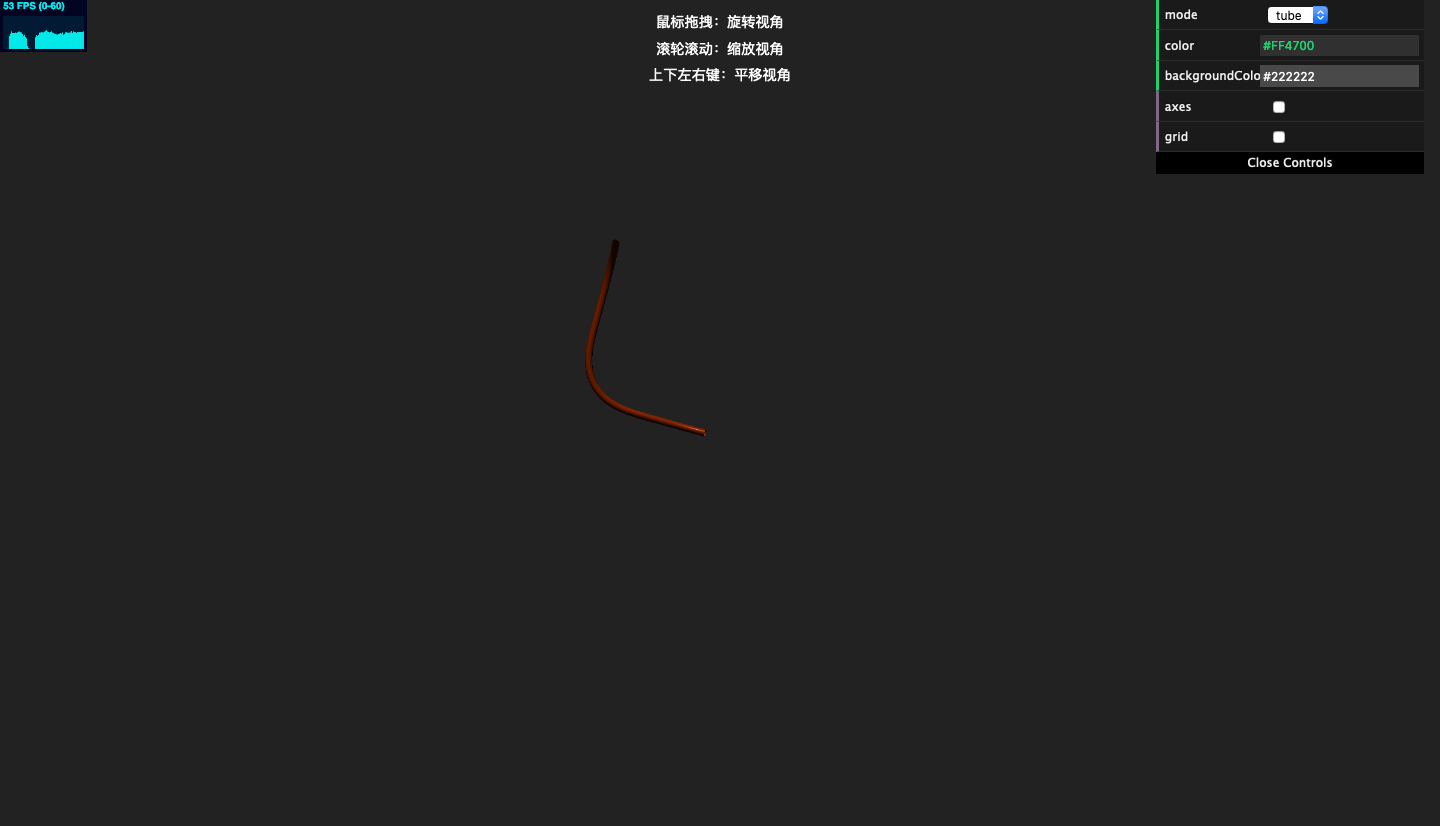
\includegraphics[scale=0.3]{change-bg-color.png}
\caption{改变背景颜色}
\label{fig:change-bg-color}
\end{figure}

\item \textbf{启用坐标轴} \\
勾选选项$axes$:

\begin{figure}[H]
\centering
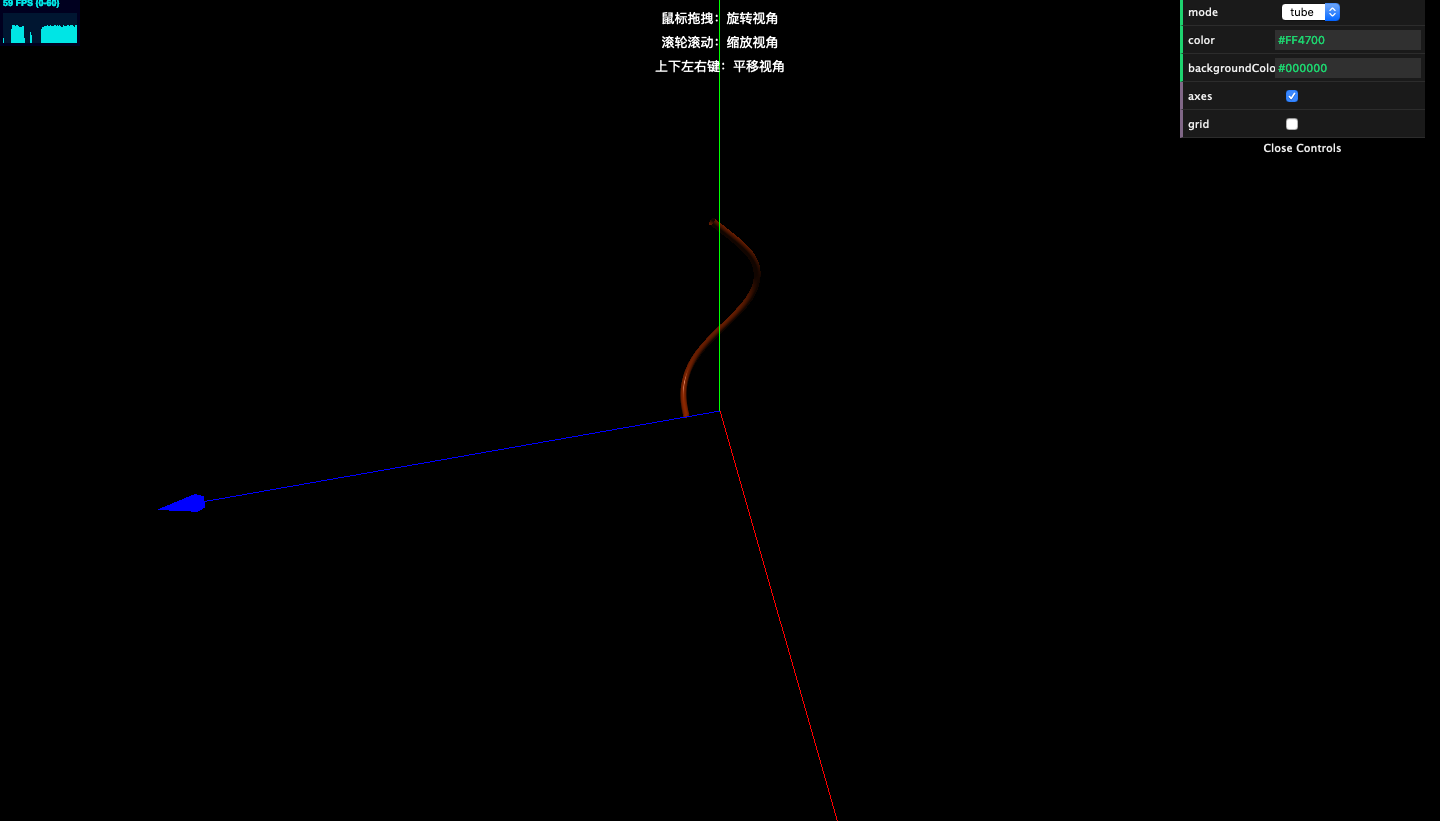
\includegraphics[scale=0.3]{tube-with-axes.png}
\caption{启用坐标轴}
\label{fig:tube-with-axes}
\end{figure}

\item \textbf{启用坐标轴和栅格} \\
勾选选项$axes$和$grid$:

\begin{figure}[H]
\centering
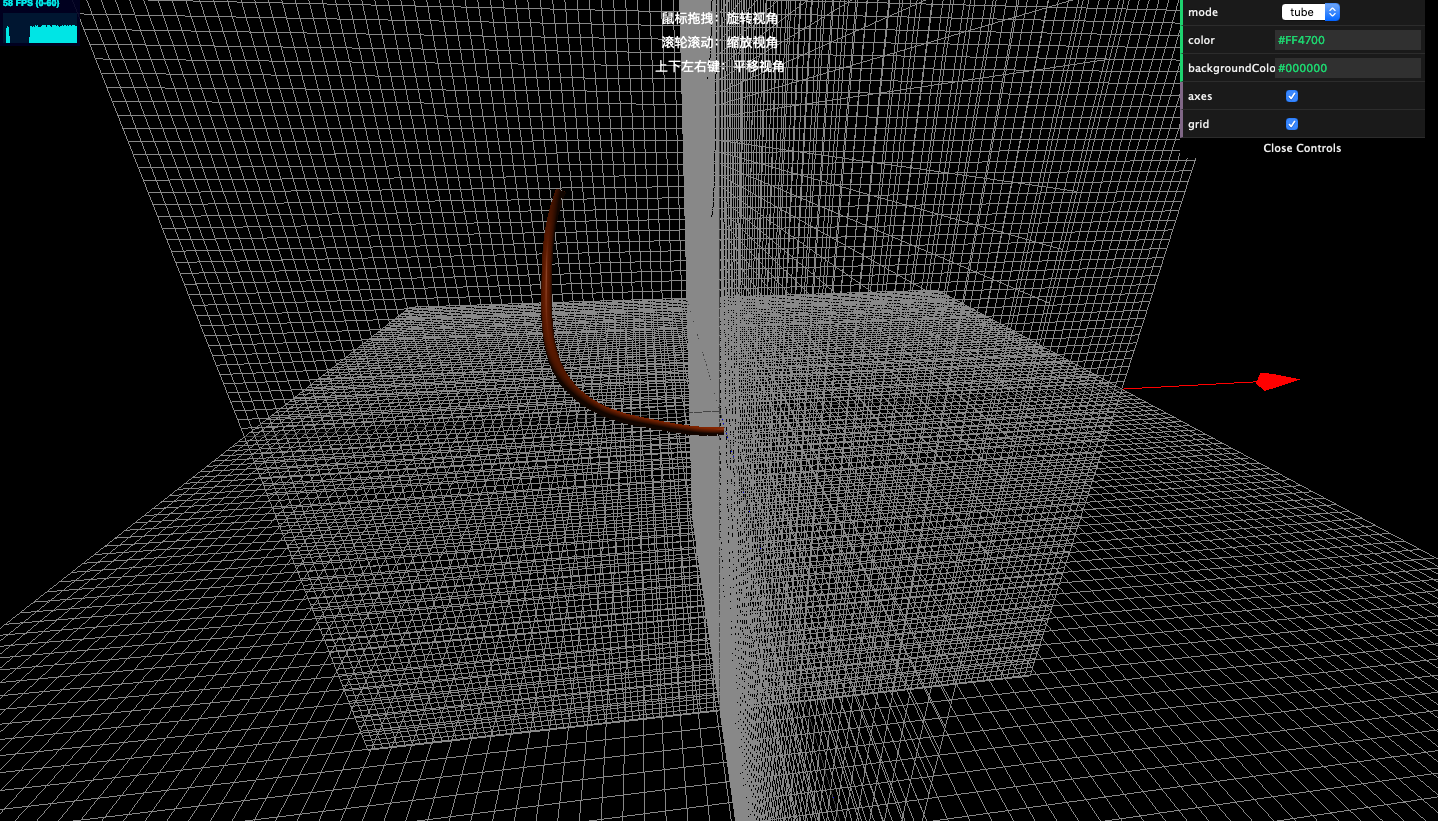
\includegraphics[scale=0.3]{tube-with-axes-grid.png}
\caption{启用坐标轴和栅格}
\label{fig:tube-with-axes-grid}
\end{figure}

\end{enumerate}

\cleardoublepage

\section{总结与展望}
本文总体来说达到了预期目标,使用的也全是当代最先进的技术。
其中WebSocket正支持着成千上万的应用;
TLS保障着整个互联网的安全;
Rust正在为Firefox添砖加瓦;
WebGL定义了下一代的三维渲染应用;
TypeScript是JavaScript社区最受欢迎的转译语言。

从架构方面来说,
渲染任务分离。服务器负责重建,所有的客户端 (浏览器)共享同一份重建数据并渲染。它
大大减少了重建算法的计算压力,仅需一个强有力的服务器完成一次重建,所有的客户端都可以共享重建结果。 
同时,它大大提升了用户的使用体验。在这种架构下,传感器、服务器和客户端即使放置在地球上有互联网覆盖的任意三点,
服务也不会中断。并且终端用户也无需从特定的机器或软件访问服务,而只需要打开任何支持WebGL和TLS
技术的浏览器,即可安全快捷地获得服务。

当然从完成度上来说,这份软件只达到了最小可用的要求,它还需要根据实际需求添加更多的功能以及对现有功能进行调整。
比如添加用户认证系统或者在渲染中更高级的动态分析。

要想构建一个成熟通用的实时三维可视化软件,还有很长的路要走,很多问题有待解决。
